\chapter{Results}
\label{cha:results}

In this 2 paths
best 80 paths States
all
1321  2166  2962  3744  4508  5235  5939

best
1294  2127  2904  3663  4395  5088  5746
\begin{figure}[H]
  \centering
  \includegraphics[width=0.5\textwidth]{results/all/states.pdf}
  \caption{Input\slash Output Process model}
    \label{fig:ioProcModel}
\end{figure}
\begin{figure}[H]
  \centering
  \includegraphics[width=0.5\textwidth]{results/all/best/states.pdf}
  \caption{Input\slash Output Process model}
    \label{fig:ioProcModel}
\end{figure}
\begin{figure}[H]
  \centering
  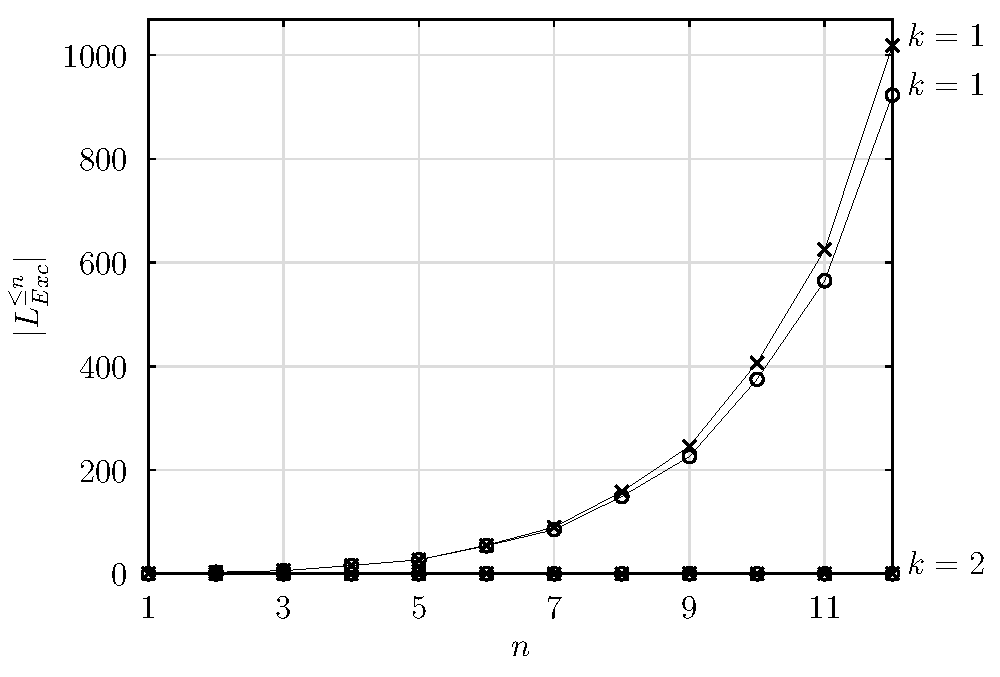
\includegraphics[width=0.5\textwidth]{results/all/exceedingLanguage-daoct-ndaao_k1-2_n12.pdf}
  \caption{Input\slash Output Process model}
    \label{fig:ioProcModel}
\end{figure}

 \section{best} 
\begin{figure}[H]
\begin{subfigure}[H]{0.5\textwidth}
  \centering
  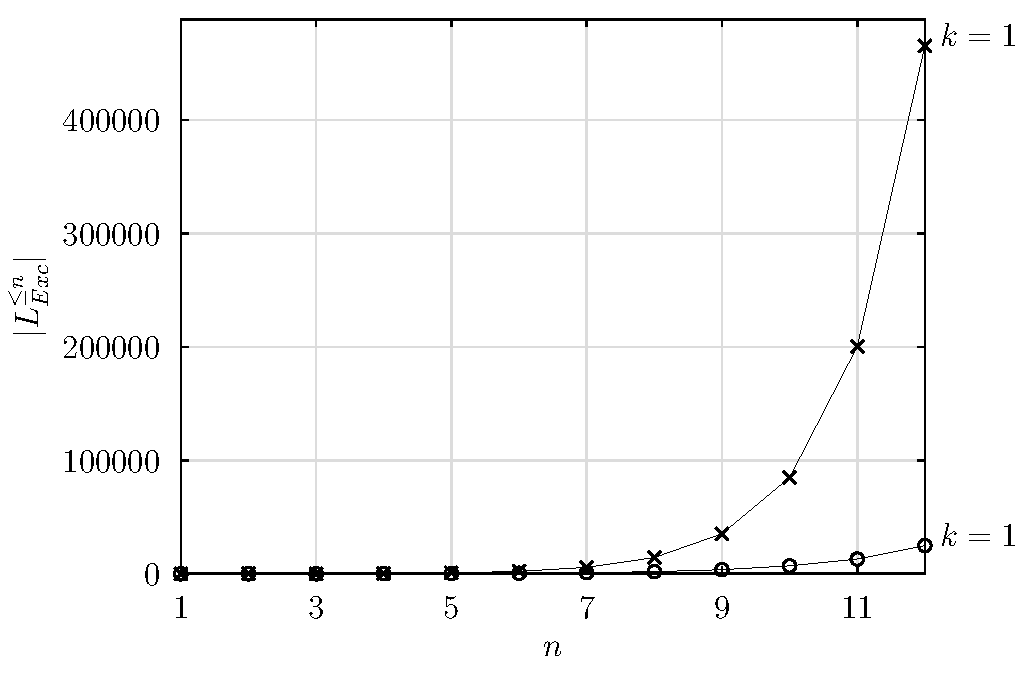
\includegraphics[width=\textwidth]{results/all/best/exceedingLanguage-daoct-ndaao_k1_n12.pdf}
  \caption{Input\slash Output Process model}
    \label{fig:ioProcModel}
\end{subfigure}
\begin{subfigure}[h]{0.5\textwidth}
  \centering
  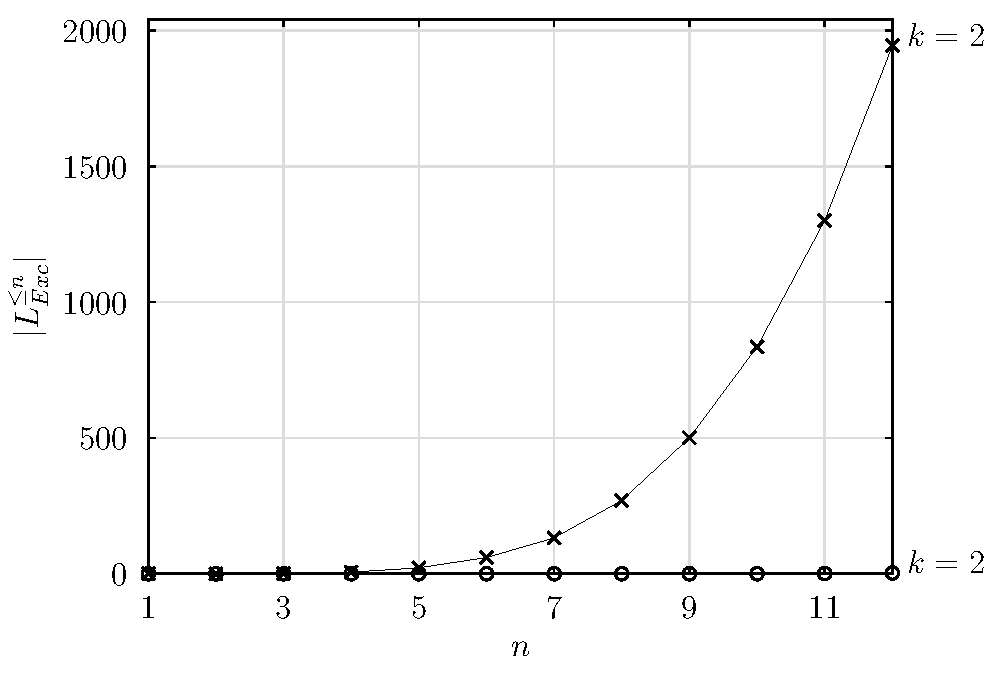
\includegraphics[width=\textwidth]{results/all/best/exceedingLanguage-daoct-ndaao_k2_n12.pdf}
  \caption{Input\slash Output Process model}
    \label{fig:ioProcModel}
\end{subfigure}
\end{figure}
\section{DAOCT}
\label{sec:results_daoct}

\section{Discussion about the identification}
\begin{figure}[H]
  \centering
  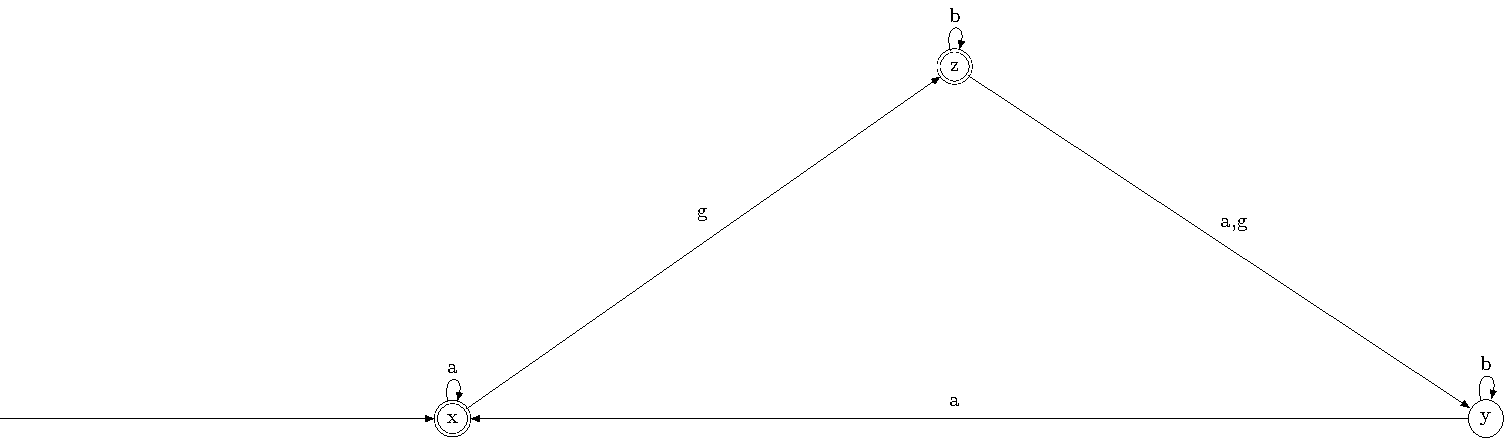
\includegraphics{results/example/example}
  \caption{Input\slash Output Process model}
    \label{fig:ioProcModel}
\end{figure}


\begin{figure}[H]
  \centering
  \includegraphics{results/example/examplek1NoArrows}
  \caption{Input\slash Output Process model}
    \label{fig:ioProcModel}
\end{figure}

\begin{figure}[H]
  \centering
  \includegraphics{results/example/example1k1NoArrows}
  \caption{Input\slash Output Process model}
    \label{fig:ioProcModel}
\end{figure}

\begin{figure}[H]
  \centering
  \includegraphics{results/example/example1k2NoArrows}
  \caption{Input\slash Output Process model}
    \label{fig:ioProcModel}
\end{figure}
% \begin{figure}[H]
%   \centering
%   \includegraphics[width=0.5\textwidth]{exceedingLanguage/example/exceedingLanguage-daoct-ndaao_k2_n7.pdf}
%   \caption{Cardinality of the exceeding language of the DAOCT (o) and NDAAO
%     ($\times$) models. $k = 1$, and $1 \leq n \leq 7$}
%   \label{fig:exceedingLangExample}
% \end{figure}


% Comparing the results of the \autoref{fig:exceedingLangExample}  with the
% example 3 from \cite{moreira2018enhanced}, we can
% observe that the exceeding language for the DAOCT model drops. This is caused by
% how the acquisition works, in this work, the plant is considered a black box, so
% instead of feeding the algorithm with the
% paths, the raw data is given, and the paths are calculated using the first
% IO\_Vector as the initial state and once this initial state is repeated other
% path 
% is created, resulting on 4 paths instead of 3. This change, can result in a
% smaller path, with no loops, diminishing the exceeding language.


% \section{Manufacture System}
% \label{sec:results_system}

% \begin{figure}[H]
%   \centering
%   \includegraphics[width=0.5\textwidth]{results/all/exceedingLanguage-daoct-ndaao_k1_n7.pdf}
%   \caption{graph}
% \end{figure}

% \begin{figure}[H]
%   \centering
%   \includegraphics[width=0.5\textwidth]{results/all/exceedingLanguage-daoct-ndaao_k2-3-7_n25.pdf}
%   \caption{graph}
% \end{figure}

% \todo{Choosing the IO\_Vector with the greatest repetition ratio as $x_0$}

% \begin{figure}[H]
%   \centering
%   \includegraphics[width=0.5\textwidth]{results/all/best/exceedingLanguage-daoct-ndaao_k1_n7.pdf}
%   \caption{graph}
% \end{figure}


% \begin{figure}[H]
%   \centering
%   \includegraphics[width=0.5\textwidth]{results/all/best/exceedingLanguage-daoct-ndaao_k2-3-7_n25.pdf}
%   \caption{graph}
% \end{figure}

% Removing I\_MAG1EMPT and I\_MAG2EMPT

% \begin{figure}[H]
%   \centering
%   \includegraphics[width=0.5\textwidth]{results/all-2_5/exceedingLanguage-daoct-ndaao_k1_n7.pdf}
%   \caption{graph}
% \end{figure}

% \todo{Choosing the IO\_Vector with the greatest repetition ratio as $x_0$}

% \begin{figure}[H]
%   \centering
%   \includegraphics[width=0.5\textwidth]{results/all-2_5/best/exceedingLanguage-daoct-ndaao_k1_n7.pdf}
%   \caption{graph}
% \end{figure}

% As we can see, the exceedingLanguage raises




%%% Local Variables:
%%% mode: latex
%%% TeX-master: "../monografia"
%%% End:
